%
% File acl2020.tex
%
%% Based on the style files for ACL 2020, which were
%% Based on the style files for ACL 2018, NAACL 2018/19, which were
%% Based on the style files for ACL-2015, with some improvements
%%  taken from the NAACL-2016 style
%% Based on the style files for ACL-2014, which were, in turn,
%% based on ACL-2013, ACL-2012, ACL-2011, ACL-2010, ACL-IJCNLP-2009,
%% EACL-2009, IJCNLP-2008...
%% Based on the style files for EACL 2006 by
%%e.agirre@ehu.es or Sergi.Balari@uab.es
%% and that of ACL 08 by Joakim Nivre and Noah Smith

\documentclass[11pt,a4paper]{article}
\usepackage[hyperref]{acl}

\usepackage{times}
\usepackage{url}
\usepackage{latexsym}
\usepackage{hyperref}
\usepackage[pdftex]{graphicx}
\usepackage{makecell}
\renewcommand{\UrlFont}{\ttfamily\small}

% This is not strictly necessary, and may be commented out,
% but it will improve the layout of the manuscript,
% and will typically save some space.
\usepackage{microtype}

%\aclfinalcopy % Uncomment this line for the final submission
%\def\aclpaperid{***} %  Enter the acl Paper ID here

%\setlength\titlebox{5cm}
% You can expand the titlebox if you need extra space
% to show all the authors. Please do not make the titlebox
% smaller than 5cm (the original size); we will check this
% in the camera-ready version and ask you to change it back.

\newcommand\BibTeX{B\textsc{ib}\TeX}

\title{A Brother Karamazov: Quantifying Morphology in Topic Modeling of Literary Russian}

\author{Virginia Partridge \\
  University of Massachusetts Amherst\\
  \texttt{vcpartridge@umass.edu}
}
\date{}

\begin{document}
\maketitle
\begin{abstract}
TODO
\end{abstract}

\section{Introduction}
Latent Dirichlet Analysis (LDA) is a widely adopted approach for unsupervised topic modeling and has been used across disciplines for exploring themes and trends in large document collections. LDA has been applied to explore the ever-growing variety of text from online platforms and social media and to analyze language changes in academic fields over time \cite{koltsova2013,mcfarland2013differentiating, vogel-jurafsky-2012-said, mitrofanova2015probabilistic}. Assuming a bag-of-words approach, LDA produces latent topics as multinomial distributions over words and each topic is viewed as being generated by a mixture of topics \cite{blei2003,steyvers2007probabilistic}.

However, what happens when words in this bag-of-words approach are themselves are complex? We turn to topic modeling on Russian, a flective language with rich paradigms for nouns, adjectives and verbs \cite{wade2020comprehensive}. Russian's inflectional morphology increases the sparsity of words' surface forms in the collection, but it's unclear to what extent this sparsity impacts the interpretability and usefulness of topics. Stemming and lemmatization treatments are typical text preprocessing steps for topic modeling, even for English, which has relatively little inflectional morphology, but there is a lack of empirical evidence that these treatments improve the models from the perspective of human interpretability or quantitative measures of topic quality \cite{schofield-mimno-2016-comparing}.

Furthermore, conflation of surface word forms may mask phenomena of interest to researchers. Topic modeling is a popular tool for exploring gender bias in corpora \cite{vogel-jurafsky-2012-said,devinney-etal-2020-semi}, and many languages, Russian included, have inflectional morphology that marks gender. By normalizing tokens to a single form, topics learned in LDA won't distinguish between Russian's feminine, masculine and neuter word forms, which may or may not be desirable depending on the domain and researchers' goals. The situation in Russian is even more nuanced that the oft cited English example ``apple'', the company, as opposed to ``apples'', the fruit \cite{schofield-mimno-2016-comparing}, as the different surface forms in Russian do share an underlying lexical word sense, but their variation results from requirements of the language's syntax.

In this work we explore baseline performance of LDA for topic modeling on a Russian literary corpus and report both quantitatively and qualitatively on the resulting topics. We first establish that topic modeling in Russian behaves similarly to English in terms of correlation with corpus metadata, regardless of the stemming or lemmatization approach. By investigating topic models produced with no morphological preprocessing step, we demonstrate that morphological features can be evident in a topic and propose ways quantify this relationship. These observations cast doubt on whether preprocessing is necessary or if its use can actually obscure information. We also present post-processing of topics as an alternative to aid with interpretability by the end users. Finally, we compare various stemming and lemmatization treatments as preprocessing the corpus and contrast this with post-processing the keywords learned by models.

\section{Related Work}
Probabilistic topic modeling has been applied on Russian text data from academic fields, social media, and Wikipedia articles \cite{mitrofanova2015probabilistic,koltsova2013,May2016AnAO}. Prior to the work on Wikipedia, little attention was given to the role of lemmatization on topic modeling in Russian, and corpora were lemmatized by default. In studying Russian Wikipedia, May et al. (2016) address the impact of lemmatization on topic interpretability via a word intrusion evaluation task, finding that lemmatization may be beneficial. However, they also suggest measuring the effects of lemmatization and do not rule out that lemmatizing in post-processing would also be effective.

The proposal for applying stemming in post-processing comes from work comparing the effects of various stemming approaches on English \cite{schofield-mimno-2016-comparing}. After comparing the relative strengths, qualitative and quantitative impacts of rule-based and context-based stemmers for English, it was concluded that stemmers do not emprically improve LDA topic models and may even hurt topic stability. Post-processing still adds value from the perspective of topic interpretability, avoiding repeating roots in topics' key word lists and  presenting users with concise results.


\section{Methods}
\subsection{Framework for Morphological Complexity}
We will first clarify terms for discussing Russian's morphological paradigms, following frameworks for quantifying morphological complexity used in linguistics and computational linguistics \cite{baerman2015intro, cotterell-etal-2019-complexity}. We draw a distinction between \textit{derivational} morphology, the process by which new words are formed through changing meaning or part of speech, and \textit{inflectional} morphology, which can be simplistically understood as verb paradigms to capture subject-verb agreement or noun declensions for case and grammatical gender. For our purposes here, we are primarily interested in the equivalence classes formed by normalizing inflectional morphology, to use an English example, conflating ``respond" and ``responds", rather than ``respond" and ``responsiveness", although aggressive stemming methods will do both conflations.

In the word-based morphology framework, inflection is captured by triples consisting of the surface form (also called wordform) $w$, a lexeme signifying the pairing of the surface for with a meaning and a slot $\sigma$, which can be understood as a set of ``atomic" units of morphological meaning, also called inflectional features \cite{aronoff1976word,sylak-glassman-etal-2015-language,cotterell-etal-2019-complexity}.
A lemma is the surface form used to look up the lexeme in a dictionary, such as the infinitive verb form. A lexeme's mapping between slots and the surface forms is not always straightforward, as multiple slots may be realized with a single surface form. This type of morphological complexity is called \textit{syncretism} and is common in Russian noun and adjective declensions \cite{baerman2015understanding,Milizia2015PatternsOS}.

There are two morphological tagsets commonly used for natural language processing of Russian. The first originates with Zalizniak's Grammatical dictionary and is used in the Russian National Corpus. A detailed explanation of these tags can be found on the website of the Russian National Corpus\footnote{\url{https://ruscorpora.ru/new/en/corpora-morph.html}}. The second is the Universal Dependency tagset, which has been applied to the Russian dependency treebank SynTagRus \cite{Sharoff2011ThePP,lipenkova-soucek-2014-converting,mcdonald-etal-2013-universal}. Both of these tagsets express slots as a list of grammatical features and the two tagsets can be mapped to each other.

\subsection{Stemmers and Lemmatization Treatments}
Following Schofield and Mimno (2016), we distinguish between rule-based stemmers, which are deterministic, but only remove endings and do not map to lemmas, and context-based lemmatizers, which rely on a dictionary of word forms paired with outputs from a part-of-speech tagger to produce lemmas \cite{schofield-mimno-2016-comparing,Sharoff2011ThePP}. Rule-based methods make no distinction between inflectional and derivational morphological processes, leading to word types, conflation classes of terms whose original surface forms may cover several lemmas.

\textbf{Truncation:} This simple baseline method trims surface forms to the first $n$ characters \cite{schofield-mimno-2016-comparing}. We try truncation with $n=5$.

\textbf{Snowball Stemmer:} This stemmer was introduced as a rigorous framework for implementing stemming algorithms for a variety of languages. We utilize the NLTK implementation\footnote{\url{https://www.nltk.org/api/nltk.stem.html}} with the original rules for Russian\footnote{\url{http://snowball.tartarus.org/algorithms/russian/stemmer.html}} \cite{snowball}.


\textbf{Mystem:} This Yandex-owned tool is the most popular lemmatizer for Russian and can be used with or without part-of-speech tags. Pairing a finite state machine algorithm for stemming with the Zalizniak Grammatical dictionary for morphological tags, this system outputs a list of possible lemmas and slots for a given token input. The system also produces probabilities for each lemma and slot based on word frequency statistics, although the source corpus for these probabilities is not clear \cite{Segalovich2003AFM}. This is not truly a context-based lemmatizer, as it does not use part-of-speech tags to disambiguate between lemmas or to assign a single slot to a syncretic surface form, but the word frequencies do represent some kind of contextual prior. We use the python wrapper for Mystem, pymystem3\footnote{\url{pythonhosted.org/pymystem3/pymystem3.html}}.


\textbf{Stanza:} This toolkit implements full neural pipelines for processing raw text, including tagging morphological features using bidirectional long short-term memory networks and lemmatizing an ensemble of dictionary based and seq2seq methods \cite{qi2020stanza}. Because each step of the pipeline depends on the output of the previous step, in order to use Stanza for morphological tagging and lemmatization, we also use its tokenization and sentence-splitting. We use the Stanza model trained on the SynTagRus treebank\footnote{\url{https://universaldependencies.org/treebanks/ru_syntagrus/index.html}}. Unlike Mystem, Stanza always produces a single lemma and morphological slot, the disambiguation step is included within the model.

Other well-known lemmatizers for Russian include TreeTagger, CSTLemmatiser, pymorphy2 \cite{May2016AnAO,Sharoff2011ThePP,pymorphy2}. We opted not to use these here due to time constraints, as they are either difficult to install (TreeTagger, CSTLemmatiser) or very slow (pymorphy2).

\subsection{Latent Dirichlet Analysis}
Latent Dirichlet Analysis uses the observed frequencies of words within documents to infer the \textit{latent}, or hidden, distributions of topics over words and topic assignments for each document. Once a number of topics $T$ is selected, the multinomial distributions $\phi_1,...\phi_T$ define the distribution of each topic $t$ over the vocabulary terms. Each $\phi_t$ is drawn from with a Dirichlet prior with concentration parameter $\beta$. Each document $d$ also has a multinomial distribution $\theta_d$ over the words in the vocabulary, also drawn from a Dirichlet prior with concentration parameter $\alpha$. Viewing LDA as a generative process, taking a joint distribution of the observed and latent variables, you are finding the $\phi_t$ and $\theta_d$ that maximize the likelihood of the corpus if you were to assign words to documents using the marginal distributions over topic assignments for the words in each document. Gibbs Sampling allows estimation of the posterior for the joint topic distribution conditioned on the observed word frequencies by directly assigning topics to each word in the corpus, iteratively sampling topics and updating topic assignments.
 \cite{steyvers2007probabilistic, blei2003,schofield-mimno-2016-comparing}.
Following Wallach et. al (2002), we will use a symmetric prior for $\beta$ and an asymmetric prior for $\alpha$ with the MALLET's Gibbs Sampling implementation to train topic models \cite{wallach2009rethinking,McCallumMALLET}.

\subsection{Evaluation metrics}
% Morphological slot entropy
% Lemma entropy
% Ratio of slots to top N key terms
% Ratio of lemmas to top N key terms
% Coherence


\section{Corpus}
The selected RussianNovels\footnote{\url{https://github.com/JoannaBy/RussianNovels}} corpus is a collection of 101 Russian literary works from the 19th and 20th centuries by 23 authors. The collection primarily consists of novels and novellas, but there are some plays (Chekhov and Sologub) and short stories (Gogol) as well. Duplicated works and multiple versions of the same work by different translators were removed. The deduplicated version of the corpus is available on Github \footnote{\url{https://github.com/ginic/RussianNovels/tree/cleanups}} with a change log.


Each work was subdivided into passages at least 500 tokens long, where tokens are determined by a simple non-whitespace pattern. This resulted in a corpus of 10,305 documents, broken down by author in figure \ref{fig:docsByAuthor} with token-level statistics given in table \ref{table:corpus}.

\begin{table*}[ht]
    \centering
    \resizebox{\textwidth}{!}{\begin{tabular}{|l|l|l|l|l|l|}
    \hline
    \thead{\textbf{Stemming/Lemmatization}\\\textbf{Treatment}} & \thead{\textbf{Unpruned number}\\\textbf{of tokens}} & \thead{\textbf{Unpruned} \\\textbf{vocabulary size}} & \thead{\textbf{Number of tokens}\\\textbf{after pruning}} & \thead{\textbf{Vocabulry size}\\\textbf{after pruning}} & \thead{\textbf{Processing time for}\\\textbf{treatment (minutes)}}\\\hline
    No treatment & 6081210 & 319459 & 3321349 & 80540 &-\\\hline
Pymystem3 & 6084073 & 80163 & 2976804 & 32648 & 4.7 \\\hline
Snowball & 6081203 & 108533 & 3070870 & 35938 & 5 \\\hline
Stanza & 6097070 & 119602 & 2980649 & 38435 & 211.2 \\\hline
Truncate to 5 & 6081210 & 59469& 3357584 & 27994 & 0.25 \\\hline
    \end{tabular}}
    \caption{Token level corpus statistics for each lemmatization and stemming treatment. Differences in unpruned token counts are due to Pymystem3 and Stanza using their own tokenization and Snowball normalizing some single characters to empty strings.}
    \label{table:corpus}
\end{table*}


\begin{figure*}[t]
    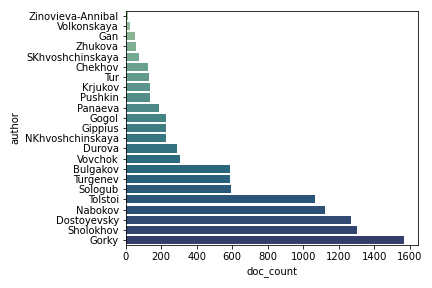
\includegraphics[width=0.5\textwidth]{document_count_by_author.png}
    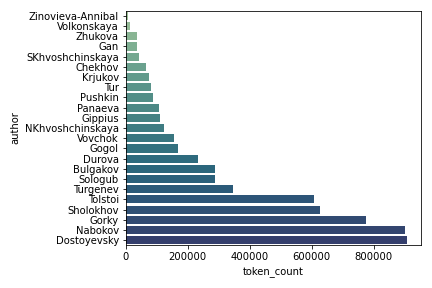
\includegraphics[width=0.5\textwidth]{token_count_by_author.png}
    \caption{The number of documents per author used to train topic models (left) and the token counts by author before pruning (right).}
    \label{fig:docsByAuthor}
\end{figure*}

\section{Results}
\section{Qualitative Observations}

\section{Conflation Treatments}
Although Stanza and Mystem are both lemmatizers, they have some functional differences
% might M

% truncation is the most agressive


\begin{figure*}[t]
    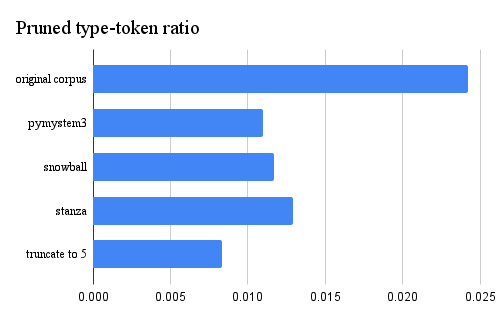
\includegraphics[width=0.5\textwidth]{pruned_type_token_ratio.png}
    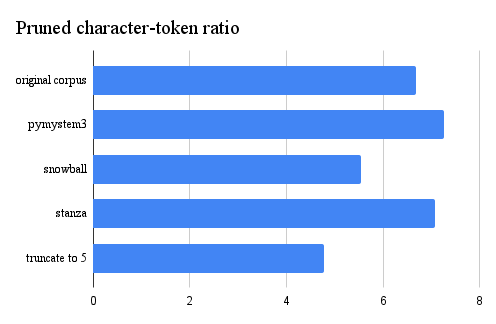
\includegraphics[width=0.5\textwidth]{pruned_character_token_ratio.png}
    \caption{The ratio of word types to tokens for each conflation treatment after the vocabulary is pruned is shown left and demonstrates the strength of conflation method in reducing the vocabulary. Character to token ratio shows lemmatization returns longer normalized strings, while stemming shortens them.}
    \label{fig:docsByAuthor}
\end{figure*}


\section{Future Work}
Standardization of stop words for more consistent comparison between metrics
Shannon-Jenson divergence
Manage vocabularies between stemmed and unstemmed corpus, account for vocabulary size when producing metrics, especially coherence
Stability


Corpora from other domains - Russian National Corpus and OpenCorpus

\bibliographystyle{acl_natbib}
\bibliography{references}
\appendix
\section{Appendix}
\label{sec:appendix}
\end{document}
